% PREAMBLE
%%%%%%%%%%%%%%%%%%%%%%%%%%%%%%%%%%%%%%%%%%%%%%%%%%%%%%%%%%%%%%%%%%%%%%%%%%%%%%%%%%%%%%%%%%%%%%%%%%%%%%%%
%%%%%%%%%%%%%%%%%%%%%%%%%%%%%%%%%%%%%%%%%%%%%%%%%%%%%%%%%%%%%%%%%%%%%%%%%%%%%%%%%%%%%%%%%%%%%%%%%%%%%%%%
\documentclass[10pt]{article}
\usepackage{geometry}                	% See geometry.pdf to learn the layout options. There are lots.
\geometry{top=1.0in, bottom=1.0in, left=1.0in, right=1.0in}                   	% ... or a4paper or a5paper or ...
%\geometry{landscape}                	% Activate for for rotated page geometry
\usepackage{fancyhdr} 			% This should be set AFTER setting up the page geometry
\pagestyle{fancy} 				% options: empty , plain , fancy
\renewcommand{\headrulewidth}{0pt} % customise the layout...
\lhead{}\chead{}\rhead{}
\lfoot{}\cfoot{\thepage}\rfoot{}
%\usepackage[parfill]{parskip}   	   	% Activate to begin paragraphs with an empty line rather than an indent
\usepackage{graphicx}
\usepackage{amssymb}
\usepackage{epstopdf}
\usepackage{booktabs} 			% for much better looking tables
\usepackage{array} 				% for better arrays (eg matrices) in maths
\usepackage{paralist} 			% very flexible & customisable lists (eg. enumerate/itemize, etc.)
\usepackage{verbatim}			% adds environment for commenting out blocks of text & for better verbatim
\usepackage{subfigure} 			% make it possible to include more than one captioned figure/table in a single float
\usepackage{algorithmic}
\DeclareGraphicsRule{.tif}{png}{.png}{`convert #1 `dirname #1`/`basename #1 .tif`.png}
\usepackage{sectsty}
%\allsectionsfont{\sffamily\mdseries\upshape} 	% (See the fntguide.pdf for font help)
%\usepackage[utf8]{inputenc} 		% Any characters can be typed directly from the keyboard, eg éçñ
%\usepackage{textcomp} 		% provide lots of new symbols
\usepackage{graphicx}  			% Add graphics capabilities
\usepackage{epstopdf} 			% to include .eps graphics files with pdfLaTeX
\usepackage{flafter}  			% Don't place floats before their definition
\usepackage{amsmath,amssymb} 	% Better maths support & more symbols
\usepackage{bm}  				% Define \bm{} to use bold math fonts
\usepackage{memhfixc}  			% remove conflict between the memoir class & hyperref
%\usepackage{pdfsync}  			% enable tex source and pdf output syncronicity
\usepackage[pdftex,bookmarks,colorlinks,breaklinks]{hyperref}  % PDF hyperlinks, with coloured links
\hypersetup{linkcolor=black,citecolor=black,filecolor=black,urlcolor=black} % black links, for printed output
\usepackage{cite}
\usepackage{mathtools}
\usepackage{subfigure}			% for putting figures "side-by-side"
%\usepackage{sidecap}			% sidecaption figures
\usepackage{wrapfig}
\usepackage{caption}
\usepackage{multicol}

%\makeatletter
%\newenvironment{tablehere}
  %{\def\@captype{table}}
  %{}

%\newenvironment{figurehere}
 % {\def\@captype{figure}}
 % {}
%\makeatother


% Title Page
\title{\textbf{CBEMD} Parallelized Molecular Dynamics in Various Thermodynamic Ensembles}
\author{Carmeline J. Dsilva, George A. Khoury, Nathan A. Mahynski,   \\
Junyoung Park, Arun Prabhu, and Francesco Ricci}
\date{}

\begin{document}
\maketitle
\begin{figure}[htbp]
   \centering
   
\includegraphics[width=2.5in]{princeton.jpg}
\end{figure}
\thispagestyle{empty}
\newpage
\setcounter{page}{1}
\pagenumbering{arabic}
\newpage

\section{Introduction}
We propose to develop a software package to perform parallelized molecular dynamics (MD) calculations for several different thermodynamic ensembles.
%
Molecular dynamics is a technique commonly used to simulate the motions of a system of interest on a microscopic level; one can then calculate macroscopic properties from the microscopic features of this system.
%
Properties such as diffusion coefficients, specific heats, and chemical potentials, which are often difficult or impossible to measure in experiment, are commonly calculated in MD.
%
It has been used to quantitatively measure the folding rate and stability of proteins using probability and enthalpic interactions and entropy through coordinate variance, to measure the melting point of a protein through constructing a sigmoidal curve tracking the root-mean square deviation from the folded structure as a function of temperature, to measure the diffusivities of atoms and larger molecules in solution and in different environments and to perform measurements at temperature extremes that are higher and lower than are experimentally convenient.
% 
This list is non-exhaustive.
%
Because of the myriad of properties that can be calculated, MD has applications in such fields as material science, pharmaceutical design, cellular biology, thermodynamics, and fluid mechanics.
%
Due to its relative simplicity and its ability to be massively parallelized, MD is a common but powerful tool for many scientists and engineers today.

\section{Background on Molecular Dynamics}
MD first initializes a system of particles, usually thought of as atoms, molecules, or another relevant (molecular-scale) group.
%
These particles have initial positions and may have initial velocities.
%
If no initial velocities are assigned, they can be computed.
%
Given an interaction potential $V (\overrightarrow{r})$ between these particles, MD integrates Newton's equation of motion, $\overrightarrow{F}=m\overrightarrow{a}$, forward in time.
%
Schematically it can be loosely illustrated as is shown in Figure~\ref{fig:workflow}.

\begin{wrapfigure}{l}{0.5\textwidth}
\vspace{-20pt}
	\begin{center}	 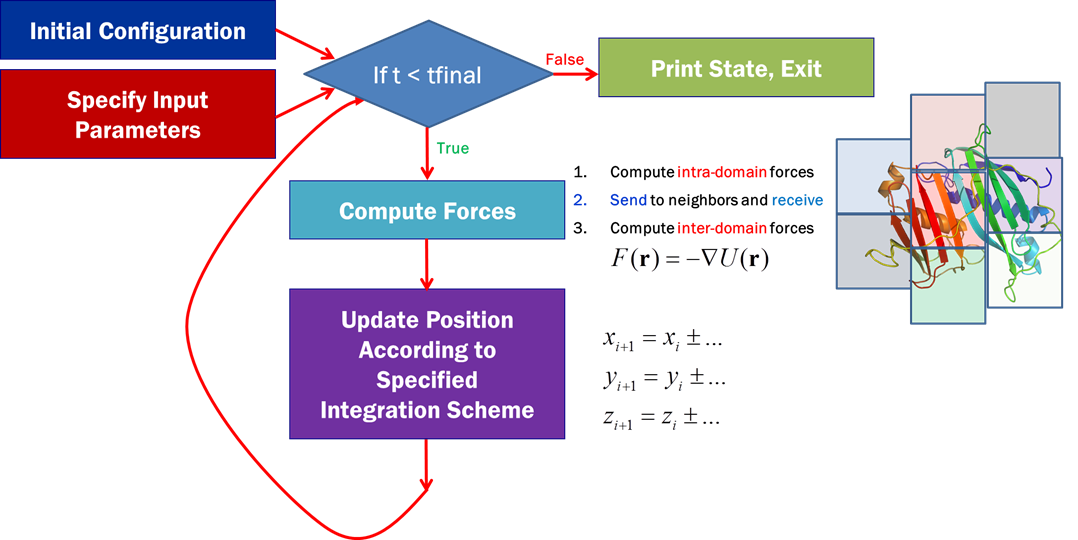
\includegraphics[width=0.49\textwidth]{workflow.png}
	\end{center}
\vspace{-20pt}
\caption{Schematic of typical workflow in a molecular dynamics simulation.}
\vspace{-10pt}
\label{fig:workflow}
\end{wrapfigure}

Thus, the flow of the program follows a well defined set of steps:
\begin{enumerate}
    \item Initialize positions and choose a timestep, $dt$
    \item Calculate the forces $\overrightarrow{F} =  -\nabla V (\overrightarrow{r}) $
    \item Numerically integrate to calculate the displacement over $dt$, using the relationships $\overrightarrow{F}=m\overrightarrow{a}$, $\overrightarrow{a} = \frac{\overrightarrow{dv}}{dt}$, and $\overrightarrow{v} = \frac{\overrightarrow{dr}}{dt}$
    \item Update positions and time
    \item Repeat from step 2 until final time
\end{enumerate}

Users of any molecular dynamics program must provide the initial configuration for the particles.
%
The user must also choose or supply the relevant potential function $V$. Different potential functions can be used to describe the system at different levels of accuracy.
%
These functions typically try to capture van der Waals interactions due to coupling of electron clouds, but can also incorporate additional effects, such as long range charge-charge interactions and solvation interactions (Debye screening effects).
%
Our project will provide an easily extensible interface so that the user can incorporate additional interactions.

For numerical stability, the timestep $dt$ is typically on the order of a femtosecond.
%
The longest simulations reported for macromolecules such as proteins are on the millisecond timescale, but such lengthy simulations can require specialized supercomputing hardware such as ANTON or GPUs.
%
Although the time integration must be done sequentially, at each step, the evaluation of the potential energy and forces can be parallelized, which is the primary reason MD has been so successful on large computer clusters.
%
Alternatively, N independent molecular dynamics simulations can be performed in parallel and often this can allow the sampling of broader space by not being trapped in local minimum.

There are many different numerical integration algorithms that have been developed, each with a slightly different purpose and numerical stability.
%
In this project, we implemented the Verlet integrator and the Andersen thermostat, which uses the Velocity Verlet algorithm.
%
Both of these integration schemes are developed specifically for molecular dynamics.

Several existing MD packages, such as HOOMD, LAMMPS, GROMACS, and NAMD, incorporate such ensembles. Members of our group use some of these codes in our every day research, but we do not know much about their internal structure. Therefore, it was a prudent exercise to develop our own codebase with a well-written interface that we can each extend for our custom applications.

\subsection{Verlet integrator}
The Verlet integrator is designed to maintain constant energy ($E$), volume ($V$), and number of particles ($N$).
%
This NVE ensemble is known in thermodynamics as the {\em microcanonical ensemble}.
% 
Such a system is a closed, isolated system, with no interactions with any external bath.
%
This scheme's equilibrium is characterized by maximum entropy.

The Verlet integrator equations are
$$ \overrightarrow{r}(t + \Delta t) = 2 \overrightarrow{r}(t) - \overrightarrow{r}(t- \Delta t) + \frac{\overrightarrow{F}(t) \Delta t ^2}{m}$$

$$ \overrightarrow{v}(t + \Delta t) = \frac{\overrightarrow{r}(t + \Delta t) - \overrightarrow{r}(t)} {\Delta t} $$

These equations can be used to update the positions and velocities of the atoms in the system, given the current positions and forces on the atoms.

\subsection{Andersen thermostat}
The Andersen thermostat is designed to maintain constant temperature ($T$), volume ($V$), and number of particles ($N$).
%
This NVT ensemble is known in thermodynamics as the {\em canonical ensemble}.
%
This scheme is setup in a way such that the system is coupled with an external heat bath that is maintained at a setpoint.
%
Its equilibrium is characterized by the minimum Helmholtz free energy, and energy is not conserved in the NVT ensemble.
%
The kinetic temperature is given by the equipartition theorem.

$$\frac{3}{2} N k_{B} T = \sum_{i}^{N_{particles}} \frac{1}{2} m_{i} \overrightarrow{v{i}}^{2} $$

In this description, the temperature setpoint specified by a user is denoted as $T_{bath}$. The system temperature is denoted as $T_{instant}$.
In the Andersen thermostat, the velocity Verlet algorithm is used for integration of the equations of motion.

$$\overrightarrow{r}(t + \Delta t) = \overrightarrow{r}(t) + \overrightarrow{v}(t)\Delta t + \frac{\overrightarrow{f}(t)}{2m} \Delta t ^{2}$$

$$\overrightarrow{v}(t+\Delta t) = \overrightarrow{v}(t) + \frac{\overrightarrow{f}(t+\Delta t) + \overrightarrow{f}(t)}{2m}\Delta t$$

In the first iteration, the forces are calculated between all of the particles. Then, knowing the velocities and forces at time t, we update $\overrightarrow{r}(t)$ to determine

$$\overrightarrow{v'}(t) = \overrightarrow{v}(t) + \frac{\overrightarrow{f}(t)}{2m}\Delta t$$

Then, the force is calculated again after the positions and velocities are updated to updated the velocities at $t + \Delta t$.

$$\overrightarrow{v}(t+\Delta t) = \overrightarrow{v'}(t) + \frac{\overrightarrow{f}(t+\Delta t)}{2m}\Delta t$$

As the particle velocities are being updated, using the equipartition theorem the temperature is calculated as

$$ T = \sum_{i=1}^{N_{particles}} m v ^{2}$$

Using this, the instantaneous system temperature can be calculated as

$$ T_{instant} = T / (3 N_{particles})$$

The velocities of particles interacting with the heat bath being applied are next updated. A Gaussian distribution with mean zero and variance $\sigma^{2} = T_{bath}$ must be constructed, denoted as $Gauss(0,\sigma^{2})$. Thus, the standard deviation of such distribution is simply

$$\sigma = \sqrt{T_{bath}} $$

Then, for each particle, a uniformly distributed random number between zero and one is calculated. If this number is less than the interaction parameter $\nu$ multiplied by the timestep $dt$, then the velocities of that particle are updated as

$$ v(i) = Gauss(0,\sigma^{2}) $$

The above algorithm proceeds until a pre-specified number of steps has completed.

\section{Code Goals and Structure}
Our code was written with the goals of generalizability and efficiency.
%
Namely we aim to produce a molecular dynamics codebase that can perform simulations
\begin{enumerate}
    \item Using different ensembles
    \item Using an arbitrary number of particles
    \item Using an arbitrary system size
    \item Using arbitrary potentials
    \item That is parallelized using MPI
\end{enumerate}
%
Our code is written as a mixture of C and C++, and utilizes many object-oriented features.
%
C++ was chosen because of its excellent memory management and ability to be object oriented.
%
C was used to create convenient structs that needed to be constantly passed around between processors (such as the MPI Atom structure). 
%
Using C structs was less expensive than using a C++ class as a container to be constantly passed around.
%
Design decisions were constantly assessed to conform to style, were made to be convenient for us to program and for others to adapt, and, for ease of understanding.

The code is optimized for small to medium-sized systems.
%
That is, a pairwise matrix of interactions exists, and we do not make use of neighbor lists in the implementation.
%
In terms of make vs. buy, it is 99.9\% make. That is, the only components of the $\approx$ 4000 lines of code produced that were not written were BOOST, MPI, and Googletests.
%

The modular class structure allows for a general coding framework, such that users can easily define their own integrators, pair potentials, and bond types.
%
We have parallelized our code using MPI.
%

We have defined various classes for the different parts of our MD simulation.
%
\begin{enumerate}
\item Atom: The atom class contains only an atom structure. This structure is passed between processors when the code is run in parallel.
\item Integrator: The integrator class is an abstract base class. It defines the implementation structure for integrators. We have implemented two integrators (Verlet and Andersen), but our code can easily be extended to other integration schemes.
\item Interaction: The interaction class is an abstract base class. It defines the interaction between two atoms, including a function pointer to different interaction potentials. We have implemented standard Lennard-Jones potential, the harmonic bond potential, and the finitely extensiable nonlinear elastic (fene) bond potential. It is optimized for small systems since it avoids bond lookup. 
\item System: The system class stores the information for the total simulation, including the box size, a list of atoms, and the interactions between atoms (stored as a matrix of function pointers to different interactions). When the code is run in parallel, each processor contains a system object that contains the atoms owned by that processor.
\end{enumerate}

We also have files ``read\_interaction.cpp'' and ``read\_xml.cpp'', which handle file I/O.
%

The flow of our code is as follows:
\begin{enumerate}
\item The code reads in the starting configuration from the user-supplied xml file, and the relevant energy parameters from the user-supplied energy file. Atoms are read from the xml file and assigned to the correct processor.
\item A system is initialized for each processor containing the relevant system parameters from the xml file.
\item An integrator is initialized on each processor.
\item The forces on each atom are calculated
\item When the code is run in parallel, the ``ghost'' atoms near the edges of each processor domain are passed to the relevant neighboring processor, and the forces between these ghost atoms and the atoms owned by the processor are calculated
\item The atomic positions are updated via the ``step()'' function for the instantiated integrator
\item Any atoms that have moved outside of the processor domain are passed to the relevant processor.
\end{enumerate}
Steps 4-8 are repeated for each timestep.
%
At each time step, the configuration of the system is output to a file.
%
This output file can be read by VMD, a molecular visualization package so a movie of the simulation can be visualized.

\subsection{Input and Output}
Our code is initialized using user-supplied xml and energy files.
%
The xml file contains information such as the positions, velocities, and masses of all the atoms in the simulation. The data can be read in any order its provided by invoking the rewind() function. A sample xml file is shown below.
%
\begin{verbatim}
<?xml version="1.0" encoding="UTF-8"?>
<hoomd_xml version="1.4">
<configuration time_step="0" dimensions="3" natoms="2" >
<box lx="10" ly="10" lz="10"/>
<position num=�2">
6.22 5 5
3.78 5 5
</position>
<velocity num="2">
0 0 0
0 0 0
</velocity>
<mass num="2">
1
1
</mass>
<diameter num="2">
1
1
</diameter>
<type num="2">
A
A
</type>
<bond num=�1">
feneA 0 1
</bond>
</configuration>
</hoomd_xml>
\end{verbatim}

The energy file contains the parameters for each interaction type in the xml file, as shown below. The parameters are the values of $\epsilon$, $\sigma$, $\Delta$, $U_{shift}$, and $r_{cut}$.
\begin{verbatim}
PPOT A A slj 1.0 1.0 0.0 0.0 2.4
PPOT A B slj 1.0 1.0 0.0 0.0 2.4
PPOT B B slj 1.0 1.0 0.0 0.0 2.4
BOND feneA fene 1.0 1.0 0.0 30.0 2.4

\end{verbatim}
It can be read in as a cascade similar to the input xml file. Its advantages include a ``factory-style'' workflow for generating the interaction matrix, which avoids constantly needing to perform ``bond lookup.'' Instead, its implemented as just a direct computation.

The shifted Lennard-Jones potential using the energy parameters, can be written as
$$
U(r) = 4\epsilon ( (\frac{\sigma}{r-\Delta})^{12} - (\frac{\sigma}{r-\Delta})^{6}) + U_{shift} ,   r - \Delta < r_{cut} $$
and the Finitely Extensible Nonlinear Elastic Model bond potential (FENE bond) can be written as
$$U(r) = -\frac{1}{2} k r_{0}^{2} ln(1 - (\frac{r-\Delta}{r_{0}} )^{2}) + U_{WCA}$$

The force on a particle can be thus calculated as 
$$ F_{i} = - \frac{\partial U}{\partial r} \frac{\partial r}{\partial x_{i}} = - \frac{\partial U}{\partial r} \frac{x_{i}}{r}$$

At each timestep, our code writes the current configuration to an output file in ``xyz'' format.
%
This file contains the positions of every atom in the simulation, and the ``xyz'' format is easily read by VMD and other molecular visualization packages.

To parse the xml file, we used the Boost C++ library to allow for discrepancies in the xml file (such as extra white space, input arguments in arbitrary orders, etc.).

\subsection{Domain decomposition}
In the final version of our code, we utilize a one-dimensional domain decomposition, where the simulation box is decomposed into vertical slabs.
%
Each vertical slab and the atoms it contains are assigned to a processor, and atoms are passed between processors as needed using MPI.
%
However, we began our project with attempting a three-dimensional domain decomposition, and it was utilized in the majority of the duration of the project.
%
Although we could not get this algorithm completely debugged by the end of this project, we will include information on the structure and implementation since it comprised a large part of our efforts.

The 3-D domain decomposition attempts to spatially split the simulation box into a number of
identical domains based on the number of processors available. 
\begin{wrapfigure}{l}{0.5\textwidth}
\vspace{-20pt}
	\begin{center}	 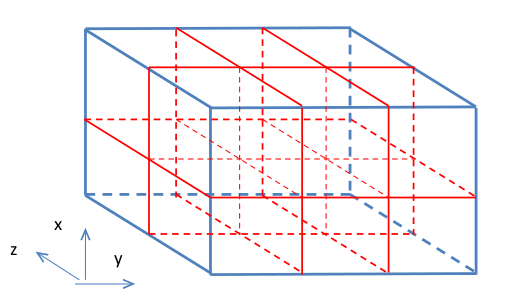
\includegraphics[width=0.49\textwidth]{ddecomp.jpg}
	\end{center}
\vspace{-20pt}
\caption{An example of the domain decomposition. The set in use is $\{2,3,2\}$ (see step 3 of the algorithm).}
\vspace{-10pt}
\label{fig:ddecomp}
\end{wrapfigure}

Each processor will then be responsible
for one domain. 
%
Parallelization will be most efficient if each processor has approximately the same load.


If we assume that the particles are uniformly distributed in the simulation box, then the most efficient way to partition the system is one in which the individual domains are as cubic as possible.
%
This is what the 3-D domain decomposition algorithm attempts to do.

Note: The 3-D domain decomposition assumes that the simulation box is a rectangular parallelepiped
with one corner positioned at (0,0,0).

The algorithm is as below
\begin{enumerate}
\item Generate the prime factorization of the number of processors available (e.g. $36 = 2 \times 2 \times 3 \times 3$).
\item Generate a set of 3 numbers by combining the factors in different ways such that the product
is still the number of processors available (e.g. for the case of 36 processors, possible sets are

$\{2,3,6\}, \{3,2,6\}, \{1,4,9\}, \{2, 1, 18\}$, etc.).
\item Divide the simulation box into domains by dividing the $x$, $y$, $z$ directions respectively into a
number of parts based on the 3 numbers in one of the sets generated in step 2. (See Fig. \ref{fig:ddecomp} for an
example)
\item Check how cubic the domains are by evaluating $diff = (d_1-d_2)^2+(d_2-d_3)^2+(d_3-d_1)^2$ ; where $d_1$, $d_2$, $d_3$
are the $x$, $y$, $z$ dimensions of a domain (since all the domains are the same size and shape).
\item Repeat steps 3-4 for all the sets generated in step 2 while keeping track of the set that resulted
in the smallest value of diff.
\item Divide the simulation box into domains based on the set which generated the smallest value of diff.
\item Assign the domains to processors by stepping through each domain in the $x$-direction from
lowest to highest and then in $y$ and then in $z$. (See Fig. \ref{fig:ddecomp} for an example)
\end{enumerate}

The code implements steps 2-4 through the recursive function gen\_sets in domain\_decomp.cpp.
The function init\_domain\_decomp in domain\_decomp.cpp starts the process from step 1 through 6
calling gen\_sets along the way.


\section{Validation}
We have compared the accuracy of the results of our simulations generated by our code to LAMMPS, a commercial/academic molecular dynamics software package. Specifically, the radial distribution function $g(\overrightarrow{r})$ was calculated over the course of a 1000 timestep simulation for a 1000 particle system. The initial coordinates and velocities of this system was input to LAMMPS and into CBEMD independently and simulated. Next, the radial distribution function was calculated for the output generated by each method.
%
The comparison is shown in Figure \ref{fig:validate}.

\begin{figure}[htb]
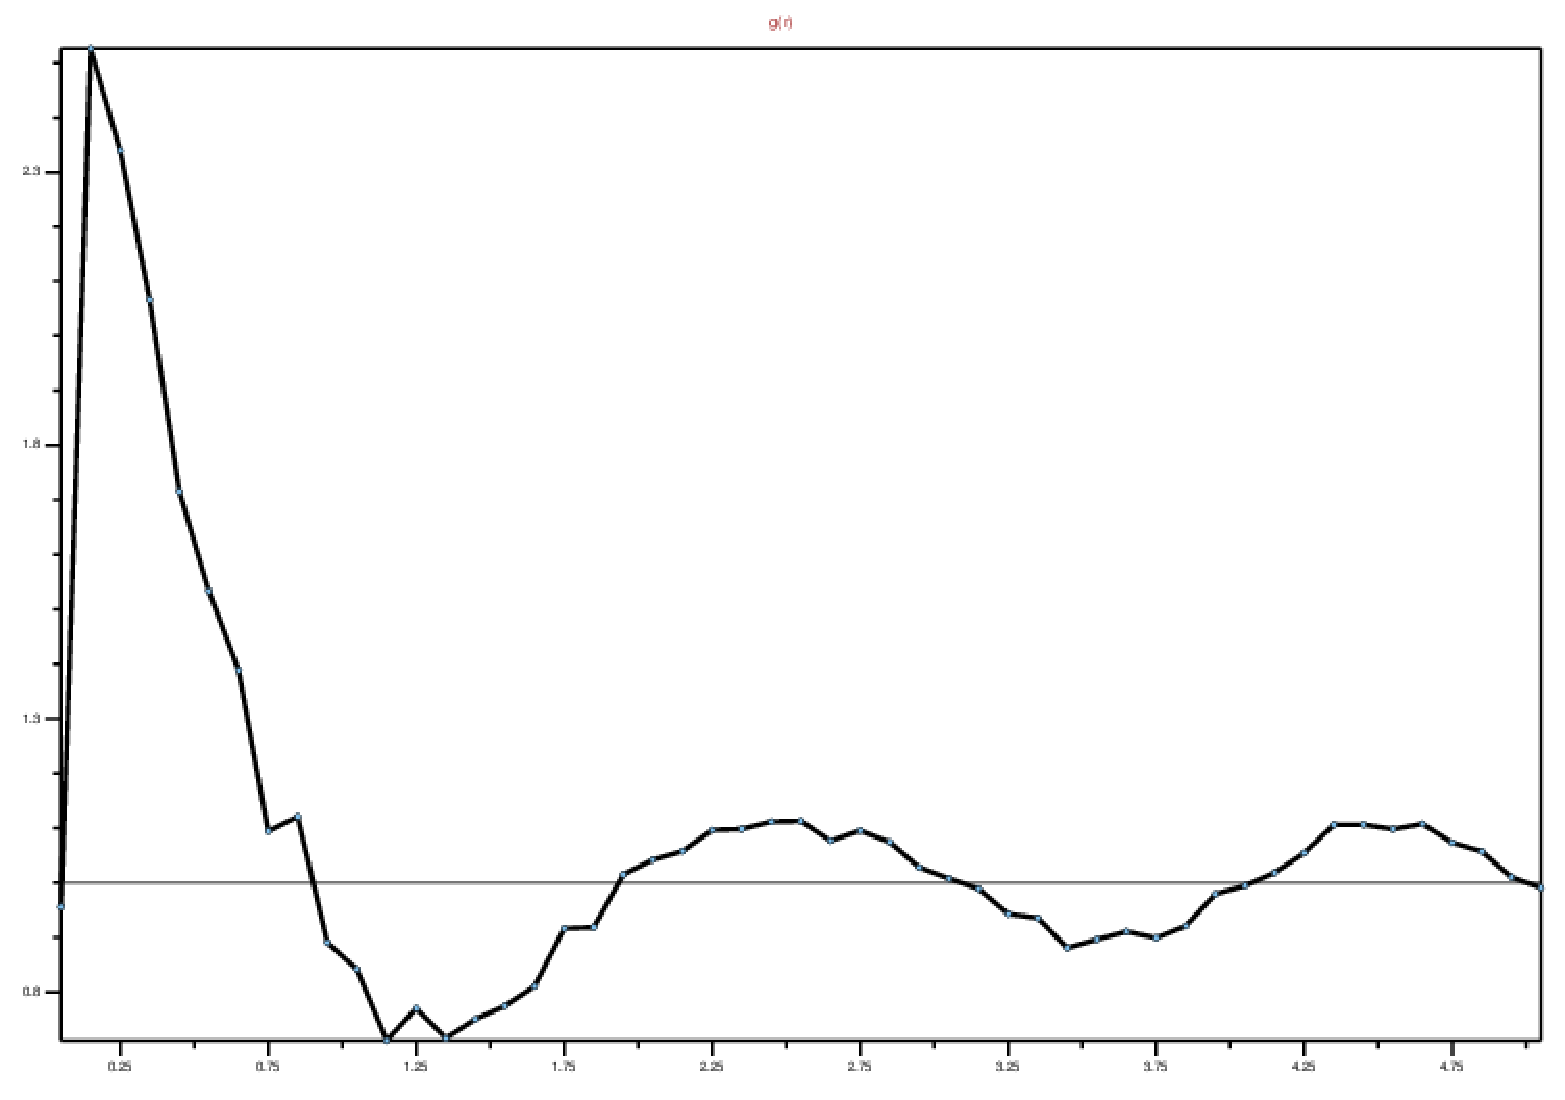
\includegraphics[width=0.5\textwidth]{gr_1000_cbemd.pdf}
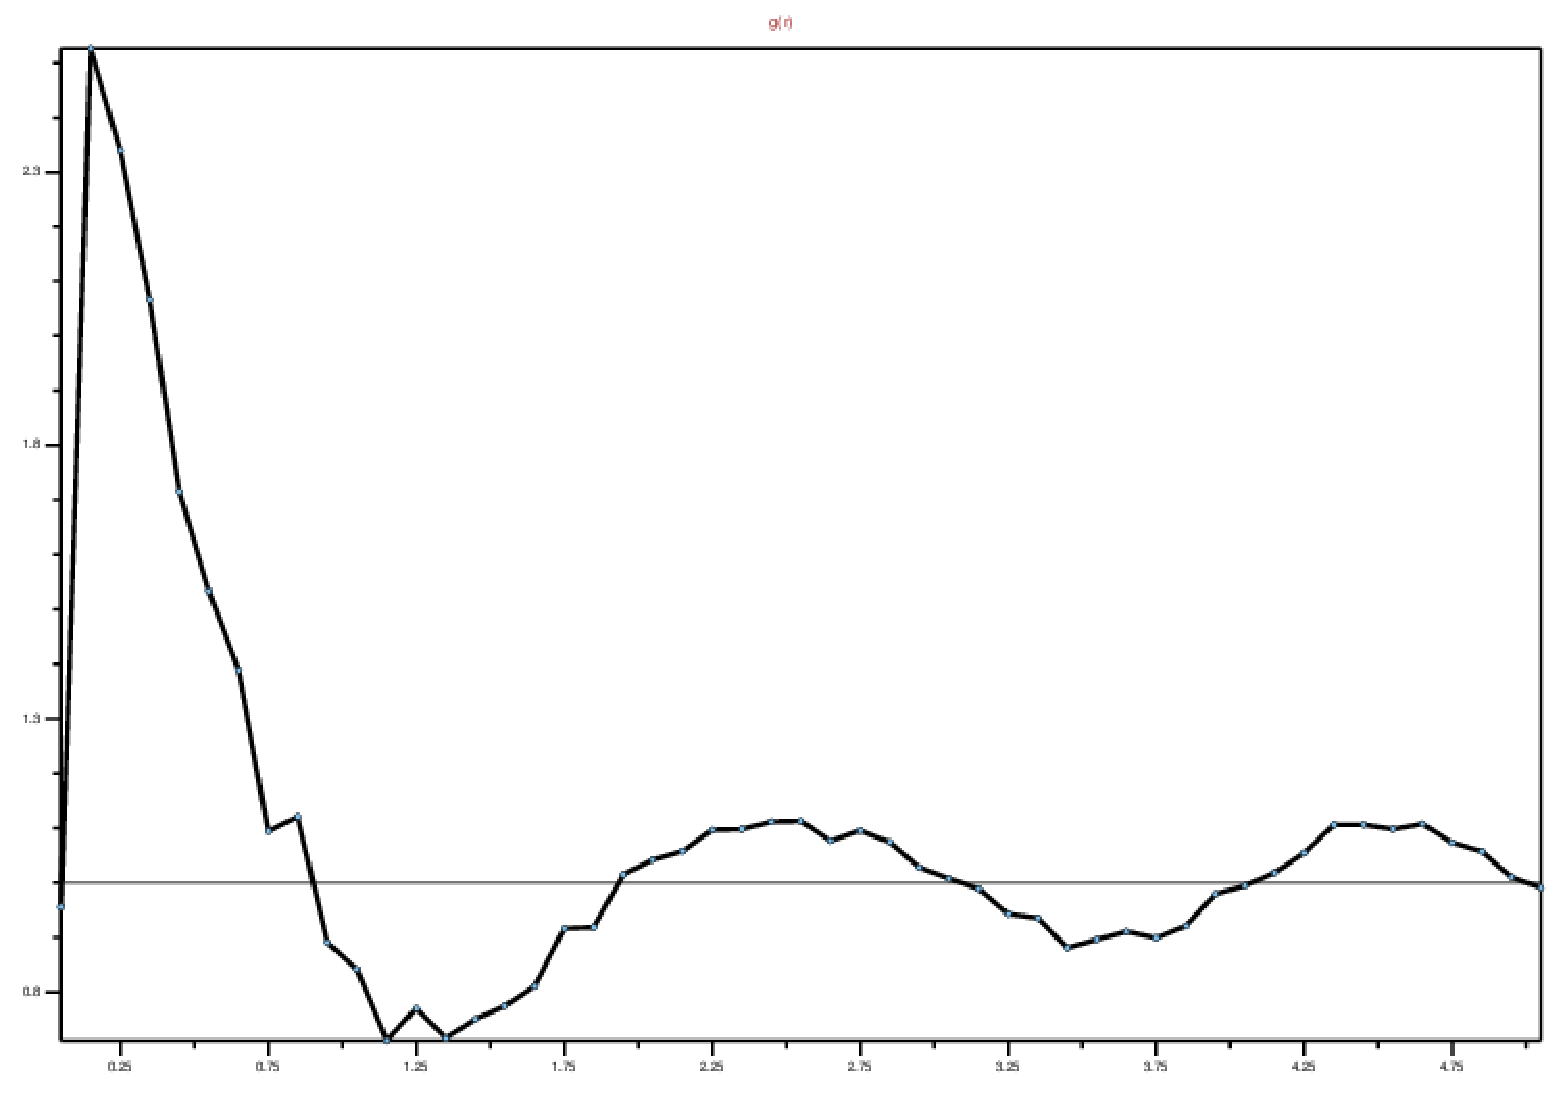
\includegraphics[width=0.5\textwidth]{gr_1000_lammps.pdf}
\caption{Comparison of the radial distribution function $g(r)$ for our code (left) and LAMMPS (right) for a 1000 atom system of Lennard Jones particles at $t=1000$ timesteps. The y-axis is the radial distribution function g(r) and the x-axis is the radius r.}
\label{fig:validate}
\end{figure}

The radial distribution function is a very important metric that describes the probability of finding a particle at a distance $r$ from a given particle, averaged across all particles. From $g(\overrightarrow{r})$, its possible to derive macroscopic thermodynamic values such as the potential energy and pressure of a system. \textit{It is evident in ~\ref{fig:validate} that the $g(\overrightarrow{r})$ produced by CBEMD is identical to that produced by LAMMPS, validating the accuracy of our program.}

\subsection{Testing}
Testing was performed using GoogleTests to test individual key components of CBEMD. 
%
The ultimate test is the exact agreement between results generated by CBEMD and that produced by the commercial package LAMMPS as shown above.
%
Nevertheless, 22 tests were written to test components of domain decomposition, calculation of the harmonic bond, fene bond, and shifted Lennard-Jones potentials, file i/o, and two-body and many body interactions. In addition, tests with domain decomposition included tests on one processor and in parallel, given an arbitrary number of processors.
\begin{figure}[htb]
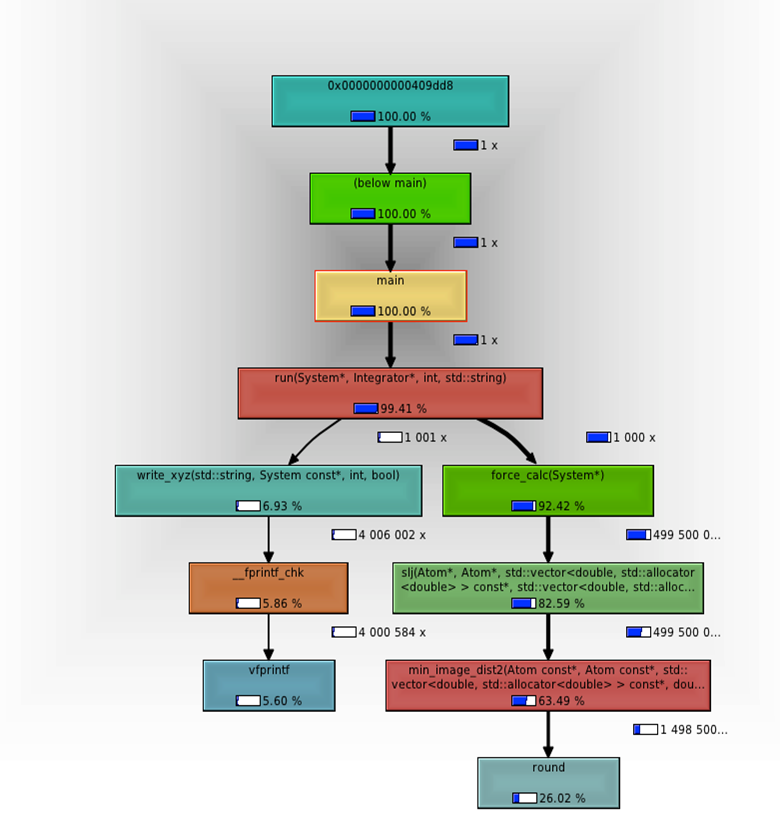
\includegraphics[width=0.5\textwidth]{serial.png}
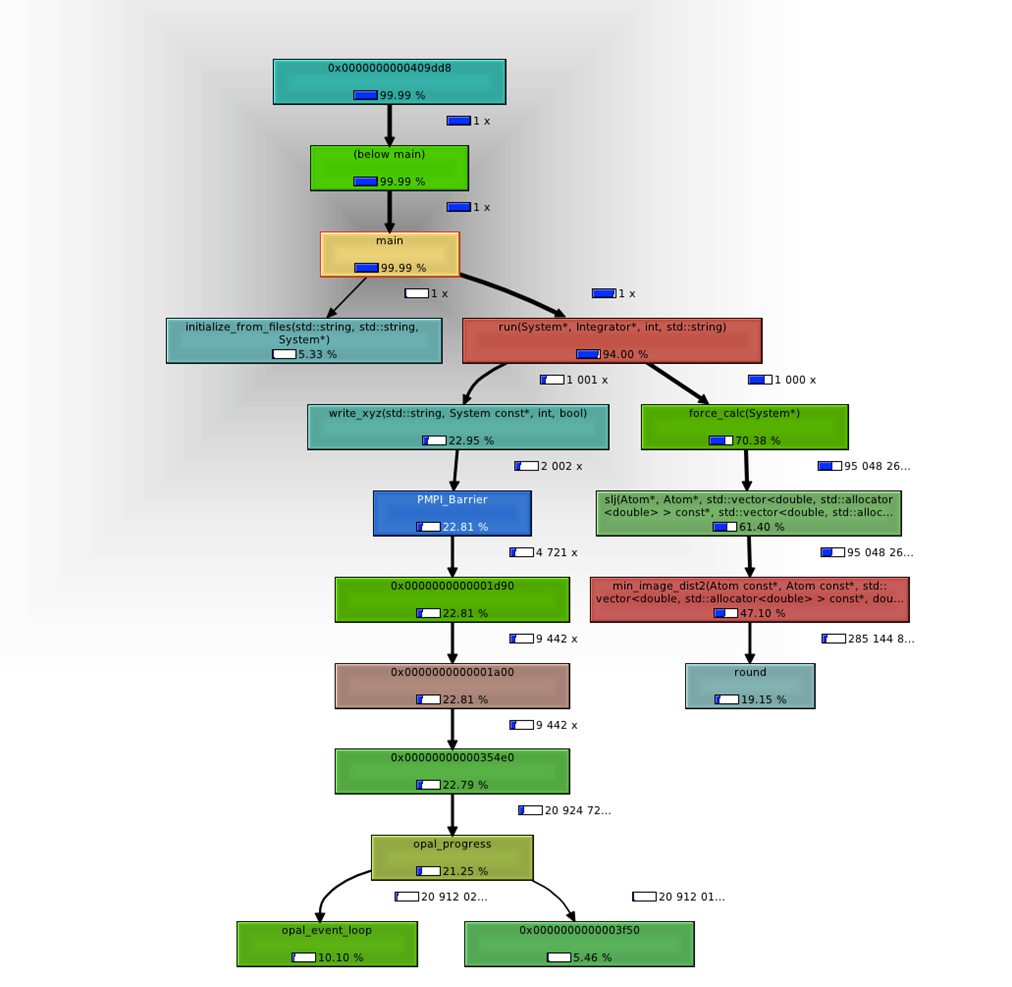
\includegraphics[width=0.5\textwidth]{mpi4procs.png}
\caption{The results from profiling using KCacheGrind while running the code in serial (left) and in parallel on four processors (right).}
\label{fig:profiling}
\end{figure}

\section{Profiling Results}
We used gprof to profile our code and highlight the computational bottlenecks (see Figure \ref{fig:profiling}).

Regions in execution that are large portions of runtime are the force-calculation, with the calculation of the shifted lennard-jones potential and the computation of the minimum-image distance taking up the majority of the time. 
%
Similarly, the use of the pow command is unnecessary when the atomic computations can be used instead.
\section{Optimization}
From the results of our profiling, we opted to optimize the ``min\_image\_dist2()'' and the ``slj()'' functions.

The ``min\_image\_dist2()'' uses the ``round'' function from the math library.
%
For dense systems, or for short simulations, this is inefficient, because most atoms are still near each other.
%
Therefore, we replaced the ``round'' function with a while loop that adjusts the distance until it is the minimum image distance.

The ``slj()'' function uses the ``pow'' function from the math library to compute $r^6$.
%
However, this function call is probably expensive and could be replaced by $r \times r \times r \times r \times r \times r$.
%

\begin{wrapfigure}{r}{0.5\textwidth}
\vspace{-20pt}
	\begin{center}	 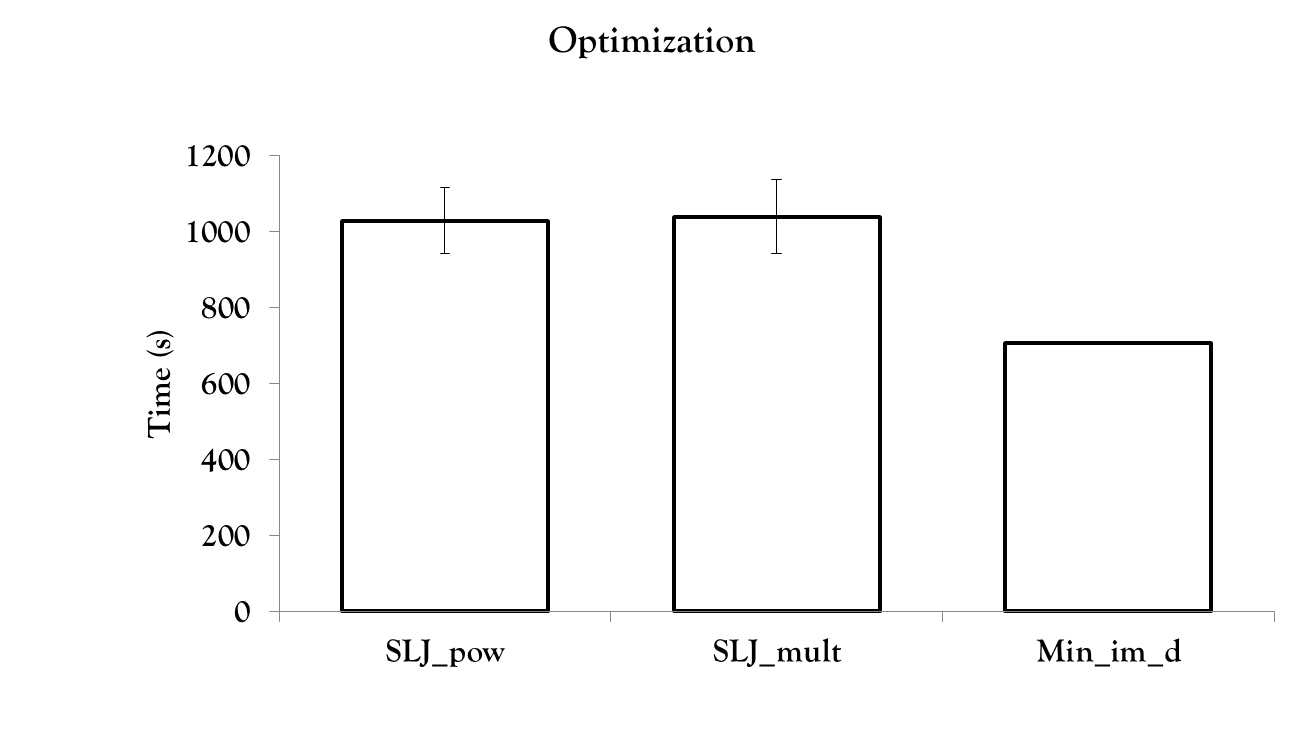
\includegraphics[width=0.49\textwidth]{optimization.png}
	\end{center}
\vspace{-20pt}
\caption{The results of optimization will be explained here.}
\vspace{-10pt}
\label{fig:optimization}
\end{wrapfigure}

Therefore, we performed several optimizations to our code to address these expensive components. The results are shown in Figure ~\ref{fig:optimization}.
%
The removal of the round function in the minimum image distance calculation reduced the time from 1000s to $\approx$ 700s, which is a dramatic reduction.
%
Conversely, comparing the runtime where the slj() function uses pow, vs. when it does the multiplications explicitly shows no improvement. 
%
This was initially unexpected. We uncovered the cause to be the use of the intel compiler for this run, which when using the optimization flag, will automatically convert uses of pow to explicit multiplications. 
%
As a result, we learned more about how compilers optimize code given to it to compile, which was very interesting.

\section{Scaling}
We looked at how the execution time of our code scaled with the number of processors.

\begin{figure}[htb]
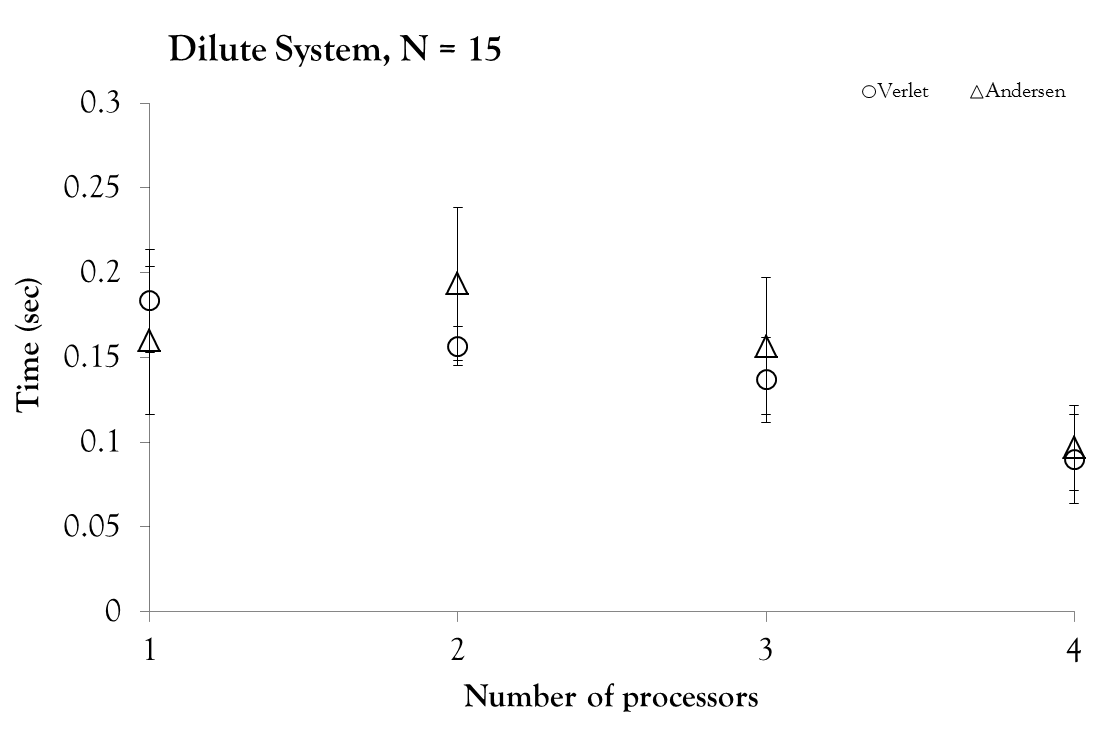
\includegraphics[width=0.5\textwidth]{scalingdilute.png}
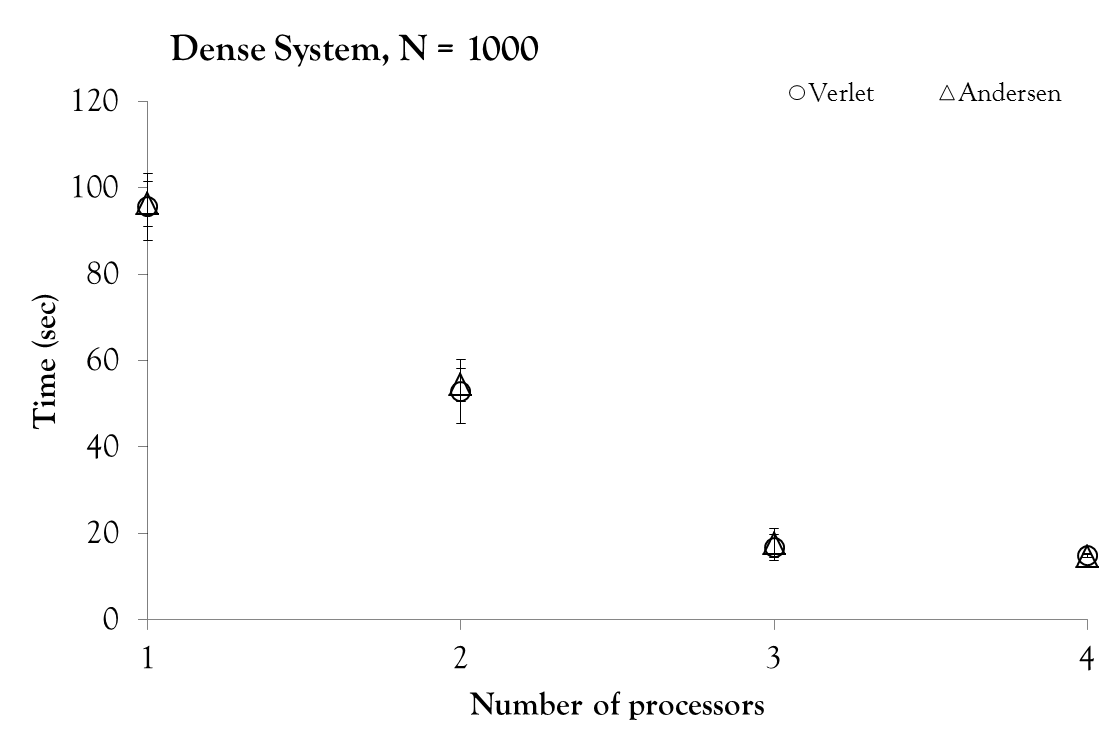
\includegraphics[width=0.5\textwidth]{scalingdense.png}
\caption{Scaling results as a function of number of processors for a dilute system (left) and a dense system (right).}
\label{fig:scalingprocs}
\end{figure}

For the dilute system, there is marginal gains achieved when increasing the number of processors used, since the system is dense and it is rare that information needs to be passed from processor to processor since the interactions are quite sparse. 
%
Conversely, for a dense system, there are many instances where information must be passed from processor to processor, so partitioning the calculation across a number of processors decreases the total time.

We next assessed scaling with system size. Theoretically, scaling should be quadratic since interactions are pairwise. 

\begin{figure}[htb]
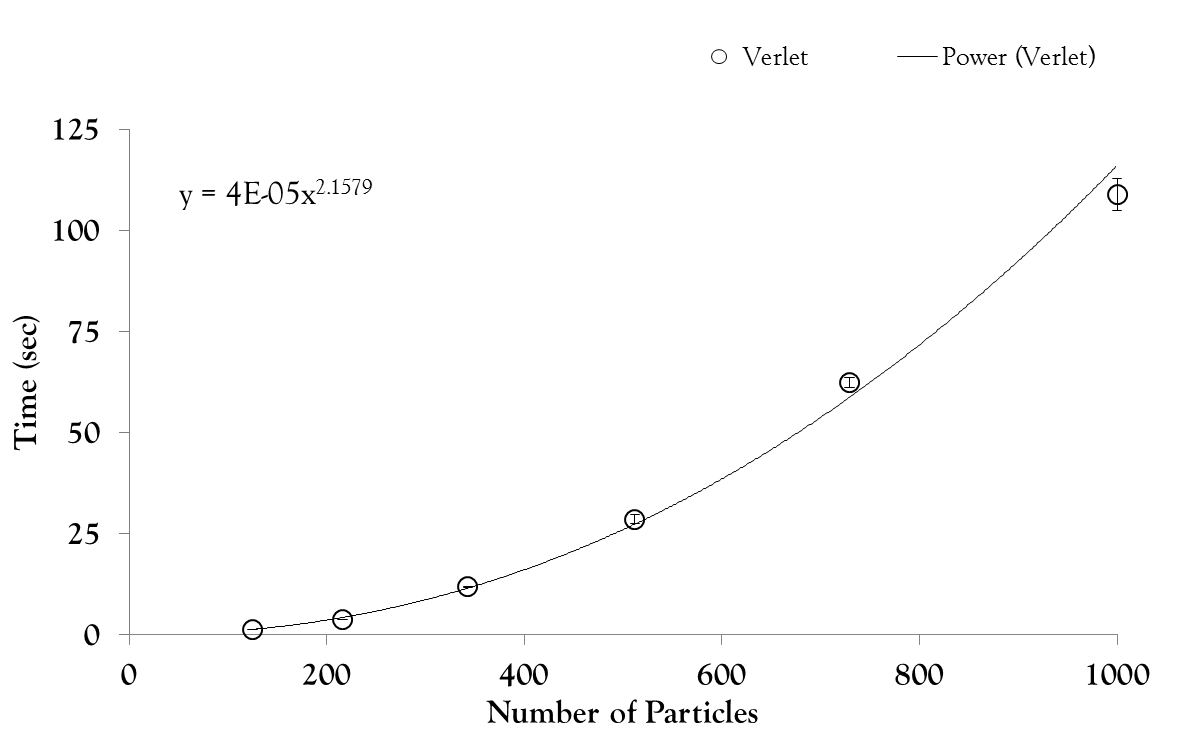
\includegraphics[width=0.5\textwidth]{scalingverlet.png}
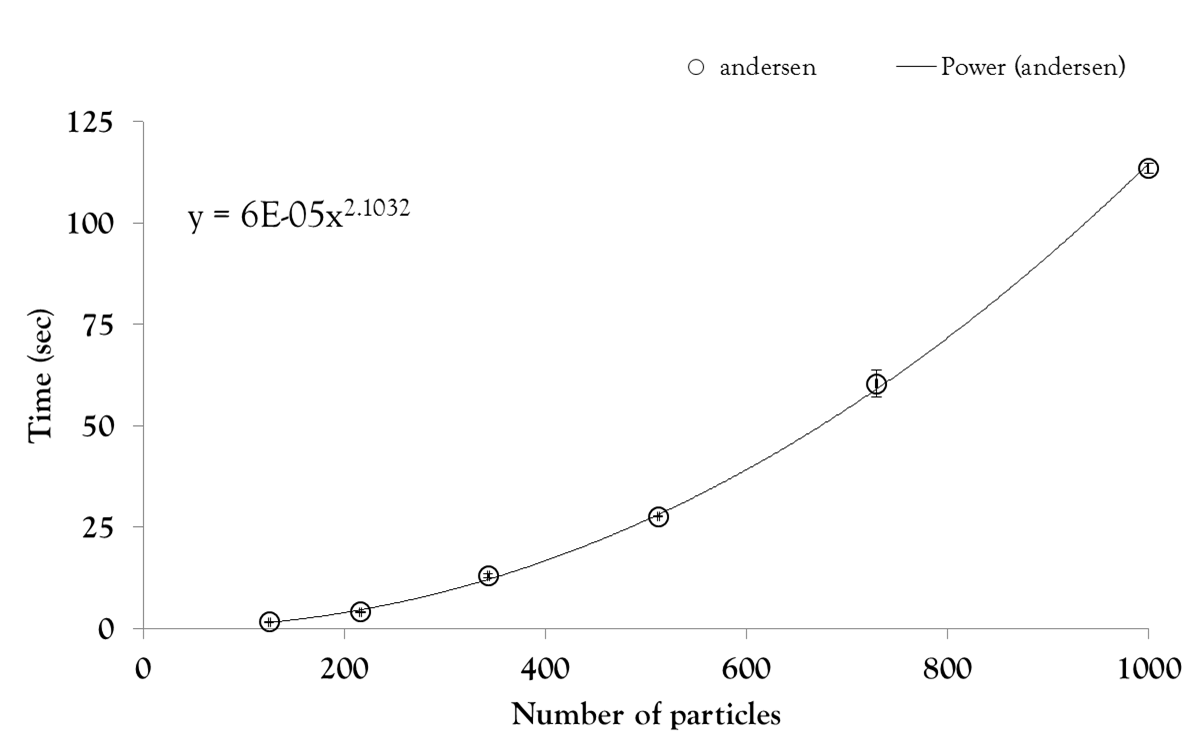
\includegraphics[width=0.5\textwidth]{scalinganderson.png}
\caption{Scaling results for integration under the N,V,E ensemble (Verlet, left) and N,V,T ensemble (Andersen thermostat, right).}
\label{fig:scaling}
\end{figure}

It is evident that the both the Verlet and Andersen integrators scale quadratically with system size, as expected. This result is promising as it indicates that the design of our program led to the expected scaling.

\section{Sample Simulation Results}

\begin{wrapfigure}{r}{0.5\textwidth}
\vspace{-20pt}
	\begin{center} 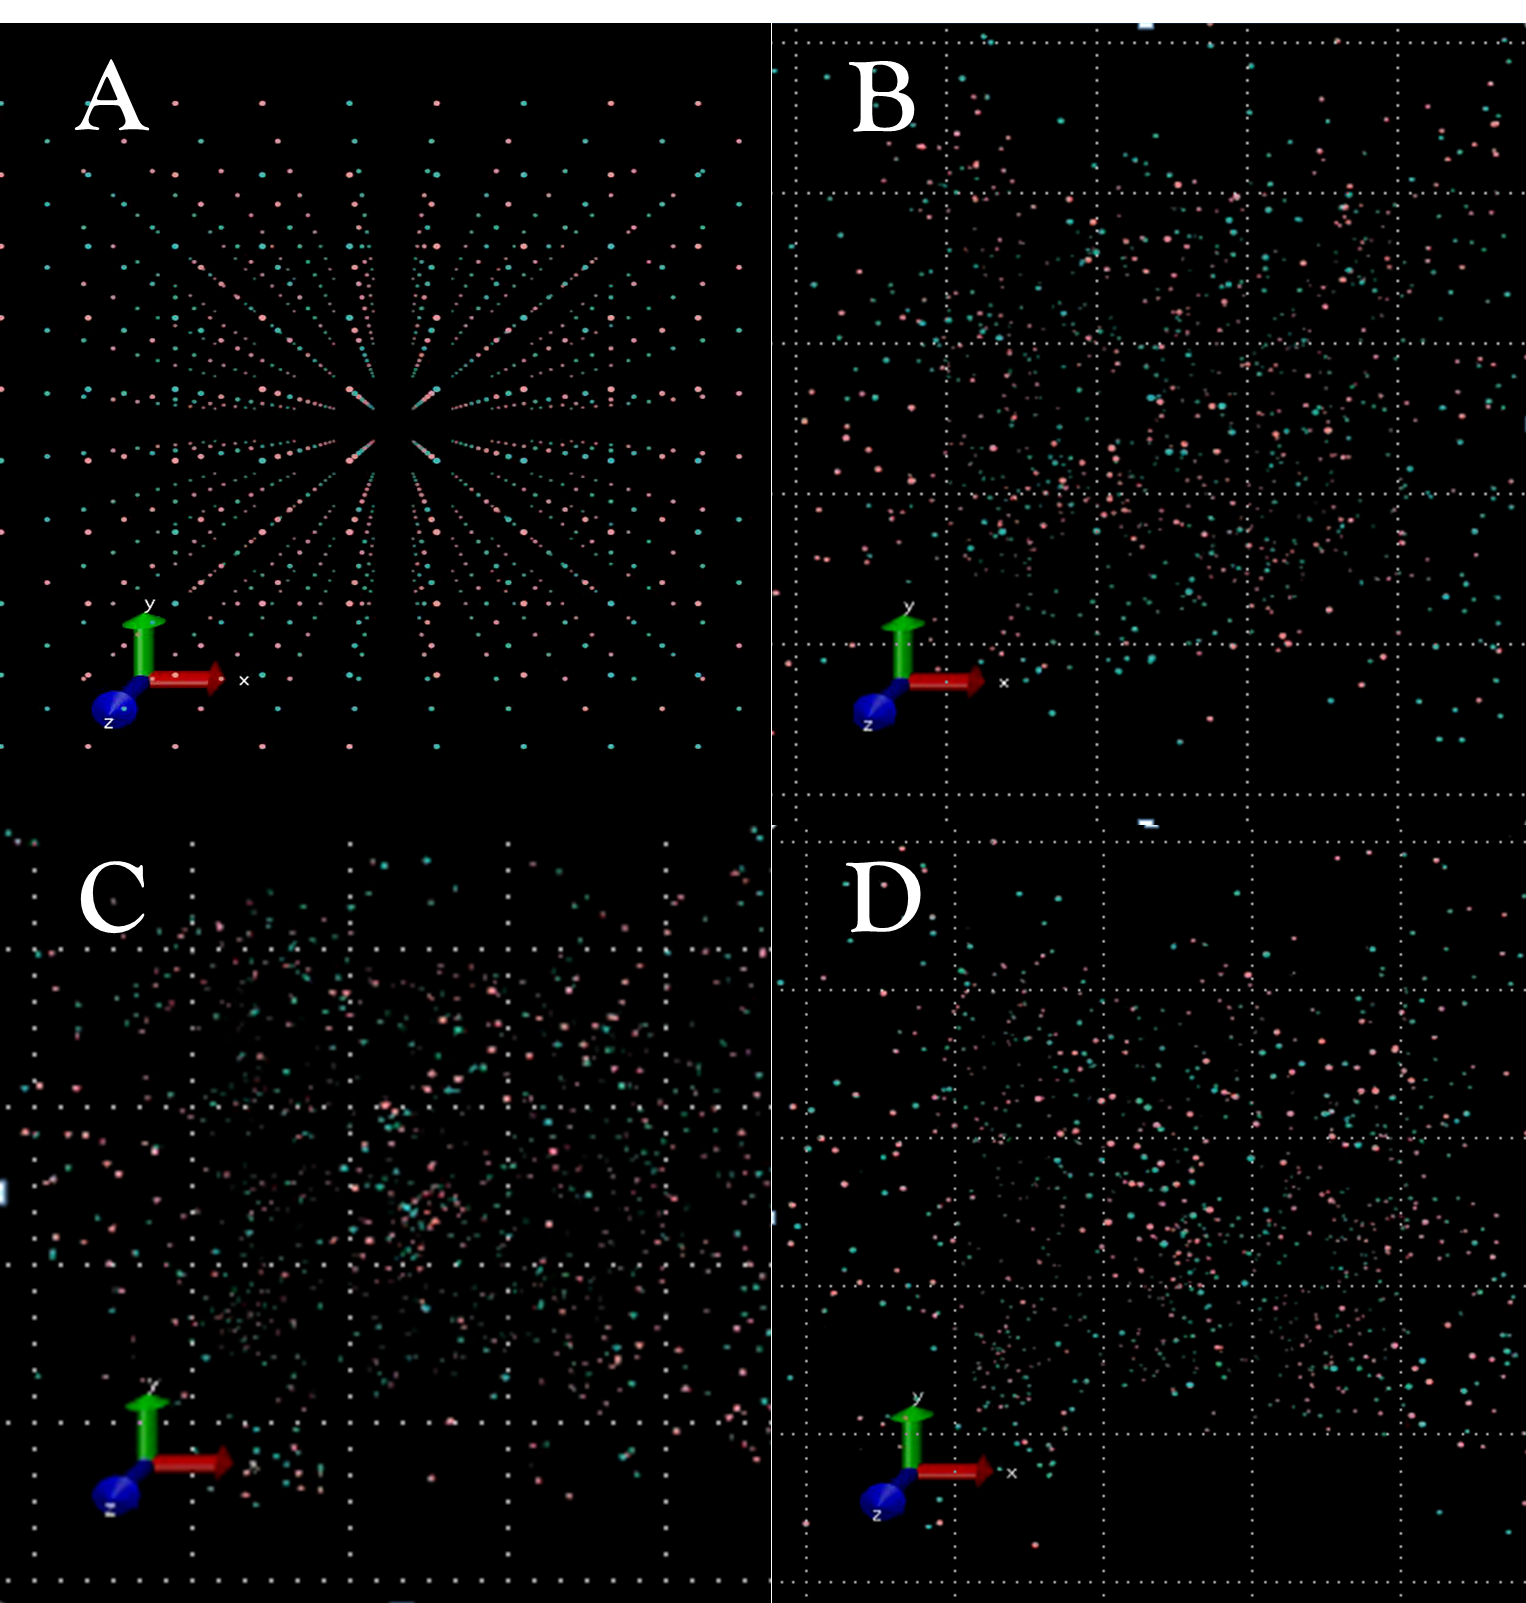
\includegraphics[width=0.49\textwidth]{snapshots.png}
	\end{center}
\vspace{-20pt}
\caption{The results of the snapshots will be described here.}
\vspace{-10pt}
\label{fig:snapshots}
\end{wrapfigure}

\section{Documentation}
All documentation of the code was done in Doxygen. A pdf file, refman.pdb is a reference manual containing full documentation of all of the functions implemented. In addition, the code comes with a README.md file that contains the instructions to compile and run the code, as well as how to run the code on the university clusters, with sample PBS scripts and sample run commands.
\section{Conclusion}

A CONCLUSION MUST BE WRITTEN.
\end{document}
